% =====================================================================
\section{Hojas de datos y referencias técnicas de los equipos}
\label{sec:datasheets}
La carpeta \texttt{Datasheets/} del entregable contiene:
\begin{itemize}
\item \texttt{Autel\_MaxiCharger\_DC\_Fast\_60-240kW\_Spec\_Sheet.pdf}: DC-1 (corrientes de entrada, conectores, certificaciones y SCCR).
\item \texttt{Autel\_MaxiCharger\_AC\_Elite\_Spec\_Sheet.pdf}: AC-1/AC-2 (UL 2594, CCID de 20~mA, corriente ajustable, NEMA~4).
\item \texttt{MDAC\_132EN\_K\_Wallbox\_7kW\_GBT\_Type2.pdf}: AC-3/AC-4 (GB/T, 32~A, normas GB/T e IEC).
\item \texttt{ABB\_Terra\_AC\_TAC-W7-G5-R-C-0\_Type2.pdf} y \texttt{ABB\_Terra\_124\_184\_NA\_Data\_Sheet\_J.pdf}: alternativas comparadas.
\item \texttt{BYD\_Dolphin\_Ficha\_Tecnica\_CR\_2024.pdf}: prueba del conector GB/T en la versión costarricense.
\item \texttt{La\_Gaceta\_Decreto\_41428\_Reglamento\_Ley\_9518.pdf}: definición de centros de recarga con referencia a INTE/IEC 61851.
\end{itemize}
Las hojas de los vehículos de mercado estadounidense, de la Zerova DS y del Ford Mobile Power Cord se consultaron en línea (ver Referencias).

% =====================================================================
\section{Memoria de cálculo reproducible}
\label{sec:memoria}
Los cálculos están en \texttt{calc/} y se ejecutan con Python~3 sin bibliotecas externas:
\begin{verbatim}
cd calc
python3 electrico.py > electrico_out.txt   # cargas, conductores, protecciones, Icc
python3 carga.py     > carga_out.txt       # energía, potencia y tiempos de carga
python3 economico.py > economico_out.txt   # presupuesto, operación y retorno
\end{verbatim}
Cada supuesto está al inicio del programa correspondiente y puede cambiarse para recalcular. A continuación se reproduce la salida del programa eléctrico. Las salidas completas de los otros dos programas están en los archivos \texttt{*\_out.txt}.

{\scriptsize\VerbatimInput{calc/electrico_out.txt}}

% =====================================================================
\section{Trazabilidad con el enunciado del proyecto}
{\small
\begin{longtable}{L{6.3cm}L{8.7cm}}
\caption{Ubicación de cada requisito del enunciado en este documento.}\label{tab:trazabilidad}\\
\toprule
\textbf{Requisito del enunciado} & \textbf{Dónde se atiende}\\
\midrule\endfirsthead
\toprule
\textbf{Requisito} & \textbf{Dónde}\\
\midrule\endhead
1. EVSE, cargador a bordo y cargador CC; CA/CC; niveles y modos & Secc.~\ref{sec:tecnologias}, primeros dos apartados\\
1. Modalidades (120~V, wallbox, condominios, CC rápida, pickups, V2V, V2L/V2H/V2G, móvil, FV, otras) & Secc.~\ref{sec:tecnologias}; Cuadro~\ref{tab:modalidades}\\
1. Verificación de pickups con salidas de 120/240~V y V2V & Combinación F-150 $\rightarrow$ Leaf, con límites (secc.~\ref{sec:tecnologias})\\
2. Ley 9518, reformas y reglamentos & Secc.~\ref{sec:ley9518}\\
2. Código Eléctrico, Decreto 36979-MEIC, edición del NEC, art. 625 & Secc.~\ref{sec:nec}; Cuadro~\ref{tab:nec}\\
2. Decreto 41642-MINAE & Secc.~\ref{sec:normativa} (alcance frente a una instalación privada)\\
2. INTE N121, N120, INTE/IEC 61851 y 62196 & Secc.~\ref{sec:normativa}\\
2. Normas IEC, SAE, ISO y UL & Cuadro~\ref{tab:normasprod}\\
2. Circuitos, cargas continuas, conductores, sobrecorriente, falla a tierra, puesta a tierra, sobretensiones, desconexión & Secc.~\ref{sec:req_inst} y \ref{sec:cc}\\
2. Distribuidora y ARESEP & Secc.~\ref{sec:distribuidora}\\
2. CFIA, municipalidad, Bomberos, Ley 7600, señalización & Secc.~\ref{sec:normativa} y \ref{sec:tramites}\\
2. Montaje, protección ambiental, cables, iluminación, emergencia & Secc.~\ref{sec:normativa}; VE-03\\
2. V2H/V2G/FV/almacenamiento & Secc.~\ref{sec:bidir}\\
3. Cuatro o más cargadores (portátil, CA, CC) & Cuadro~\ref{tab:cargadores} (7 equipos)\\
3. Cinco o más vehículos (automóvil, SUV, pickup) & Cuadro~\ref{tab:vehiculos}\\
3. Conectores, compatibilidad por versión y mercado, adaptadores & Secc.~\ref{sec:compat}; Cuadro~\ref{tab:matriz}\\
3. Selección y justificación & Secc.~\ref{sec:seleccion}\\
4. Puntos de carga (cantidad, tipo, potencia, ubicación) & Cuadro~\ref{tab:puntos}; VE-01\\
4. Plano con cargadores, estacionamientos, tableros, cableado, accesos, cotas y leyenda & VE-00 y VE-01\\
4. Unifilar & VE-02\\
4. Energía, potencia efectiva y tiempo de carga & Secc.~\ref{sec:calc_carga}; Cuadro~\ref{tab:tiempos}\\
4. Conductores y canalizaciones & Secc.~\ref{sec:cond}; Cuadro~\ref{tab:conductores}\\
4. Protecciones & Secc.~\ref{sec:cc}\\
4. Detalles de montaje & VE-03\\
4. Cuadro de cargas, de equipos, BOM, presupuesto, costo de operación & Cuadros~\ref{tab:cargas}, \ref{tab:equipos}, \ref{tab:bom} y \ref{tab:operacion}\\
4. Emergencia, mantenimiento, ampliación y cambios en la instalación & Secc.~\ref{sec:ampliacion}\\
5. Análisis y viabilidad & Secc.~\ref{sec:analisis}\\
6. Conclusiones & Sección de conclusiones\\
7. Prompts de IA & Anexo~\ref{sec:ia}\\
\bottomrule
\end{longtable}}

% =====================================================================
\section{Datos del sistema eléctrico existente reutilizados del Proyecto 2}
\begin{figure}[H]
\centering
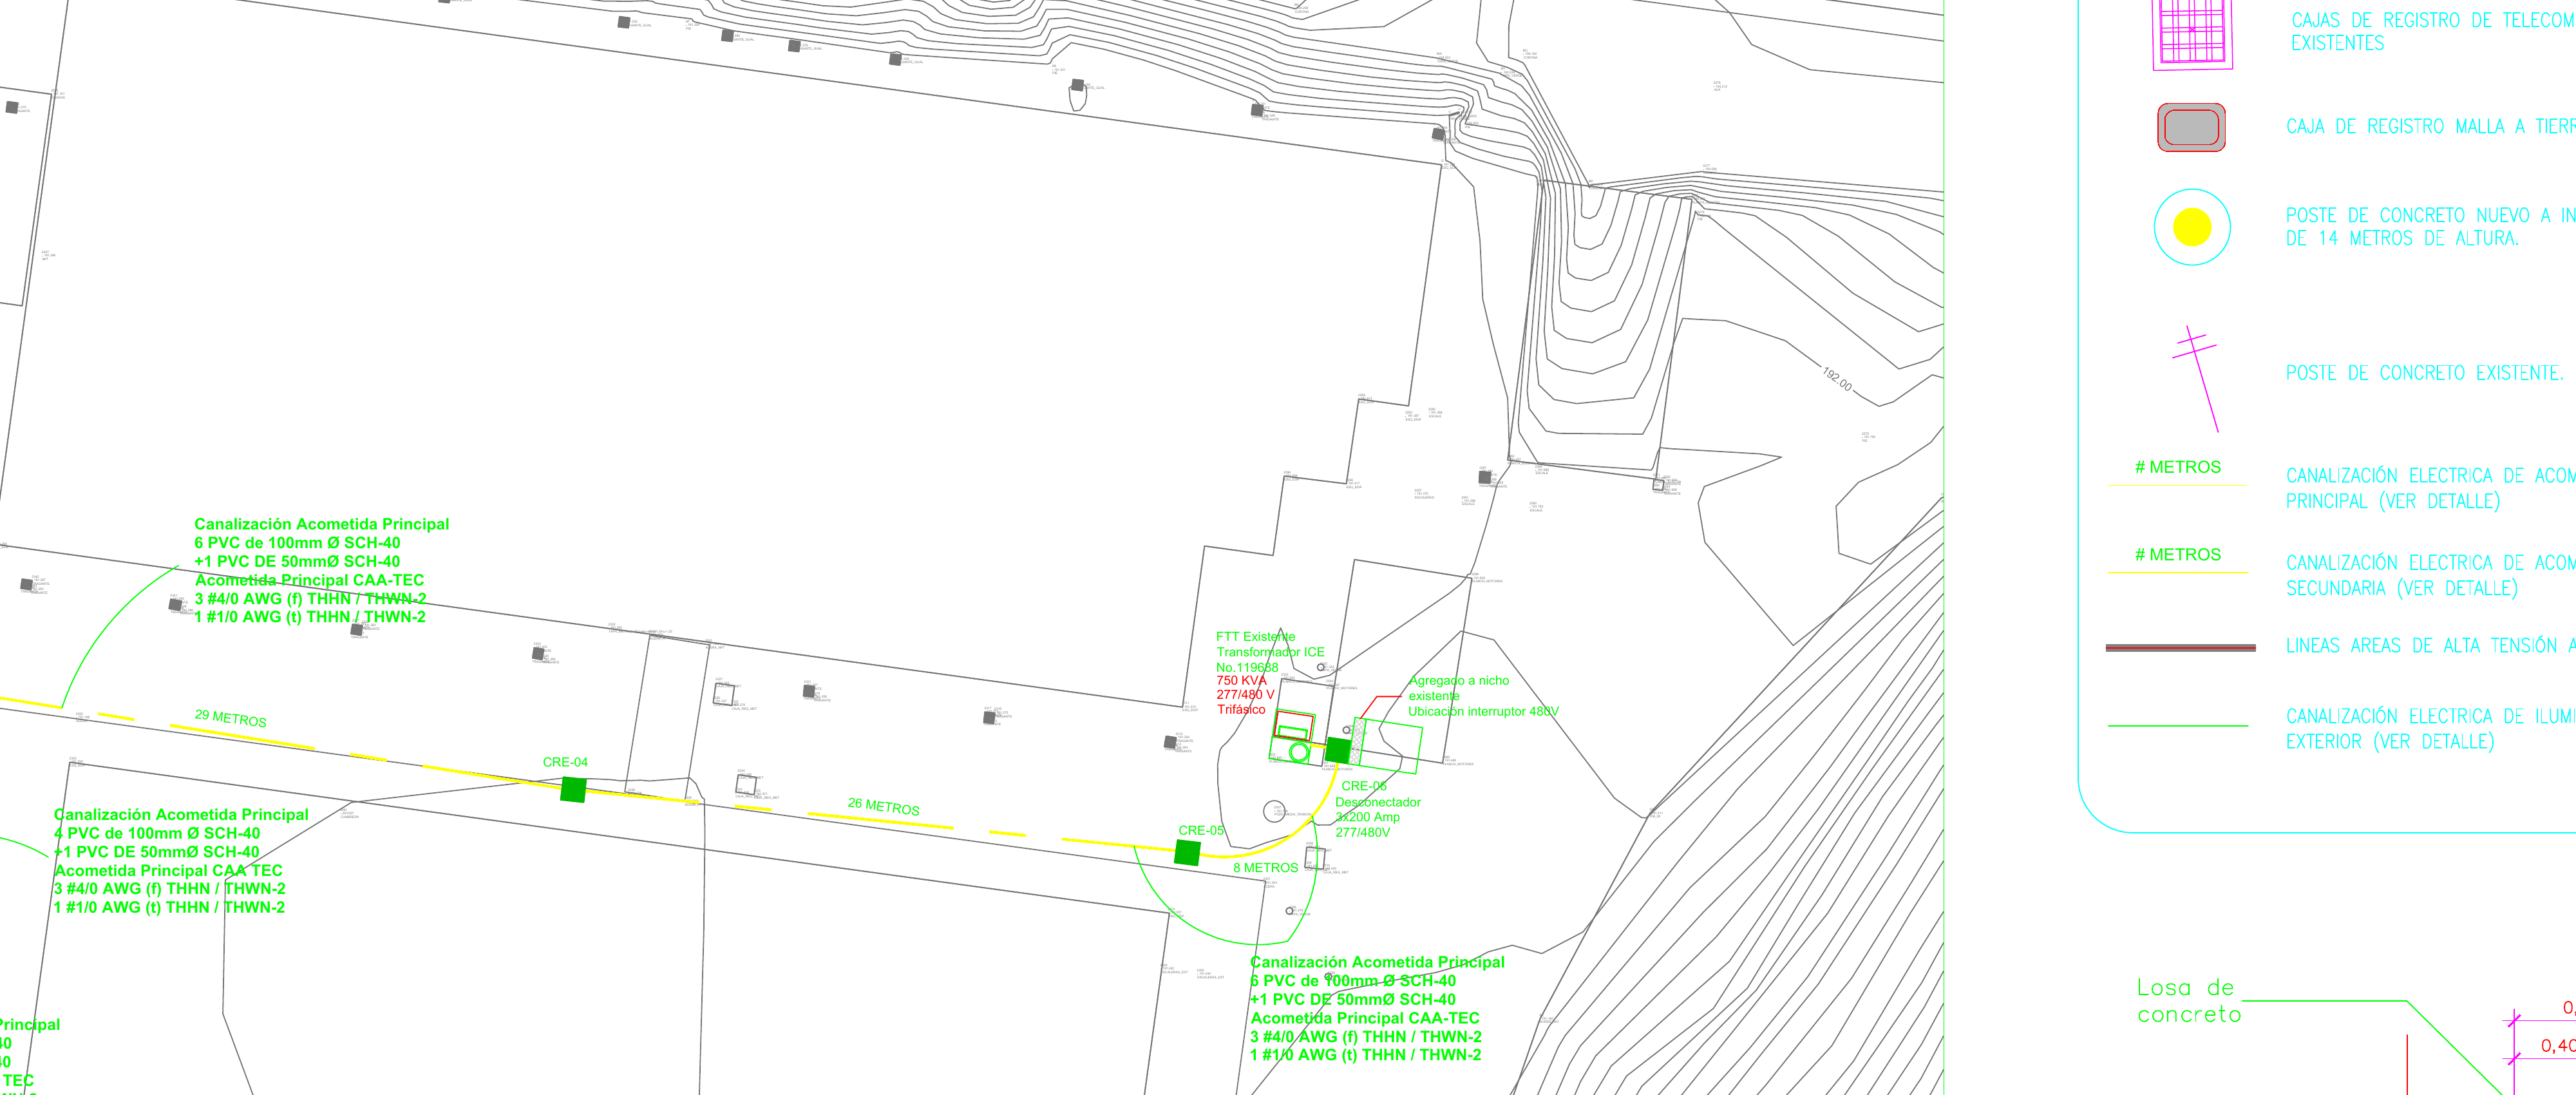
\includegraphics[width=0.92\textwidth]{figuras/acometida.png}
\caption{Lámina E01 (as-built del CAA): transformador del ICE N.\textsuperscript{o} 119688, nicho del interruptor de 480~V y canalización de la acometida existente \cite{p2}.}
\end{figure}
\begin{figure}[H]
\centering
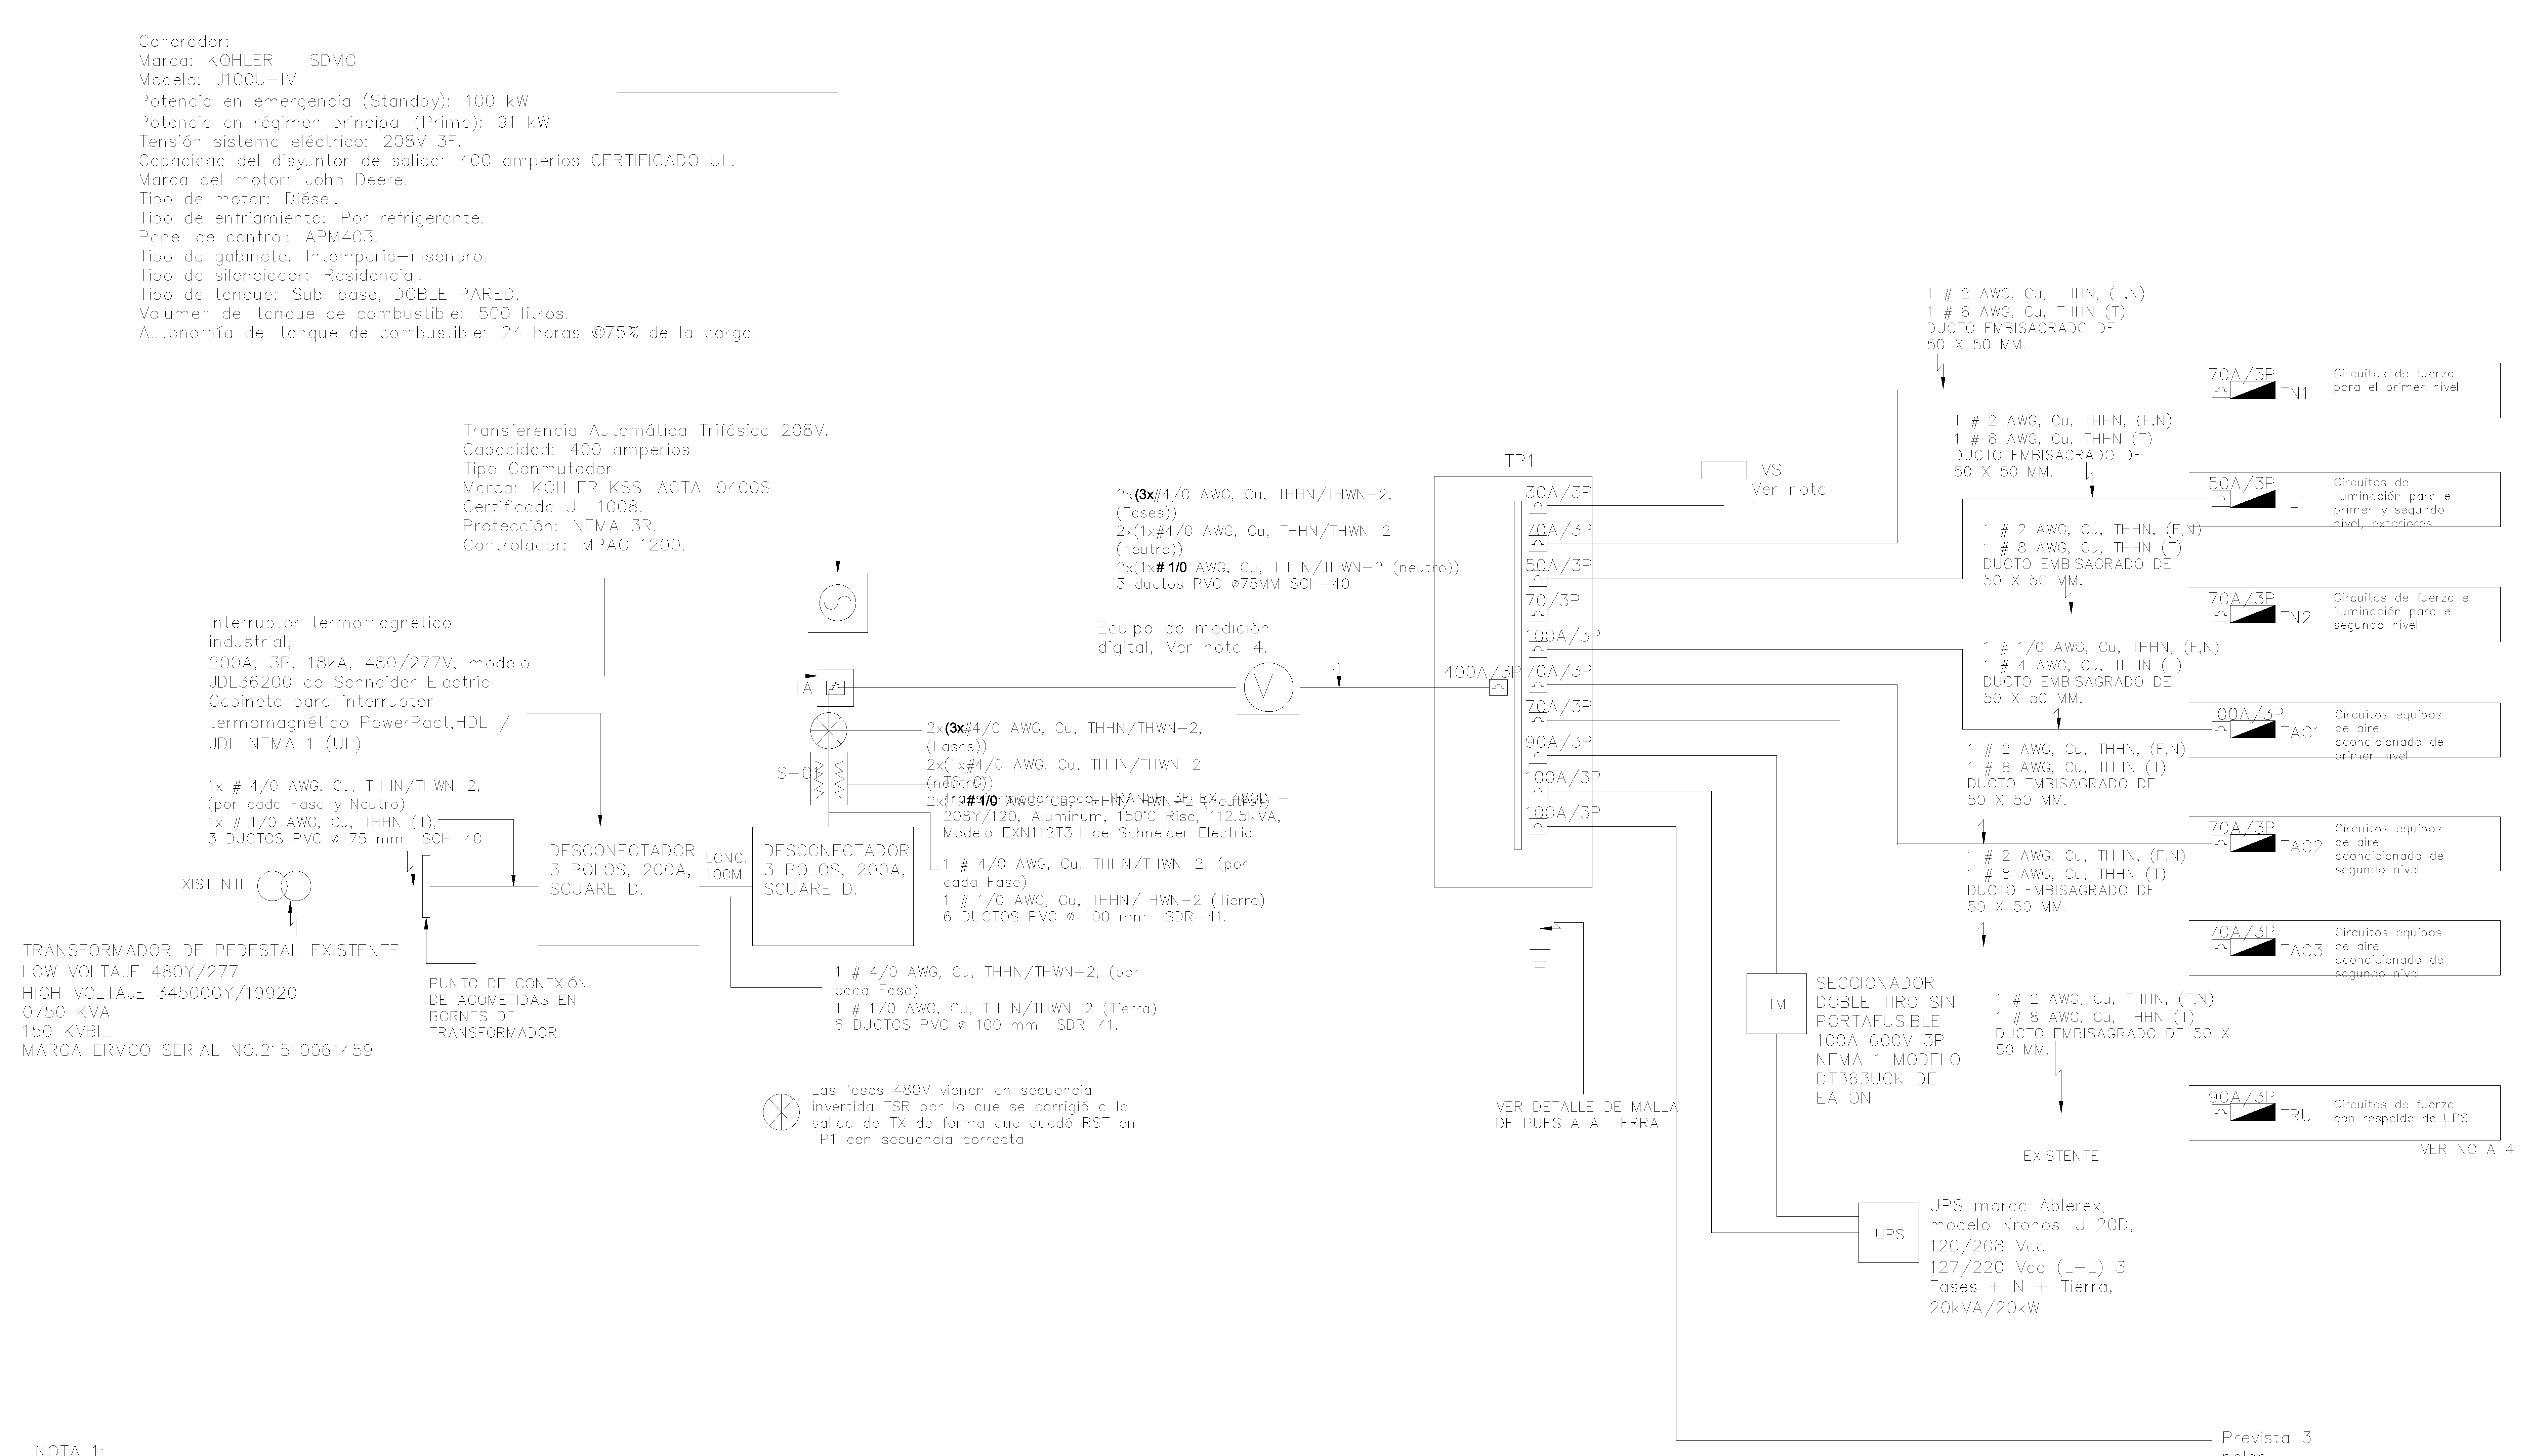
\includegraphics[width=0.92\textwidth]{figuras/unifilar_existente_bn.png}
\caption{Unifilar existente del CAA (E07): la estación no toma carga de TS-01 ni del TP, sino de un servicio nuevo en el nicho del transformador \cite{p2}.}
\end{figure}
